\section{Maquettes du programme}

\subsection{Maquettes de l'application android}

  \begin{figure}[htbp]
  \begin{center}
    \leavevmode
    \subfloat[Première page de l'application Royal\_Scanner]{%
		\label{}
		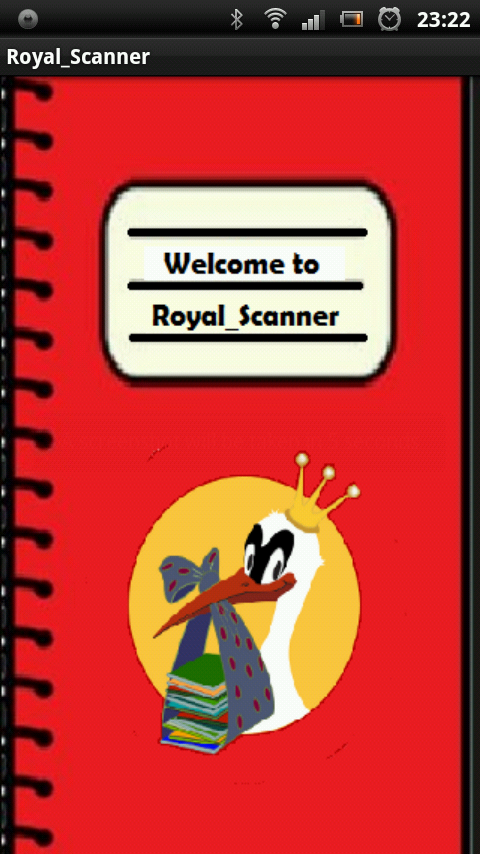
\includegraphics[height=7cm]{../Image_Royal_Scanner/First_Screen_Royal_Scanner.png}}
    \hspace{4cm}
    \subfloat[Menu de l'application Royal\_Scanner]{%
		\label{}
		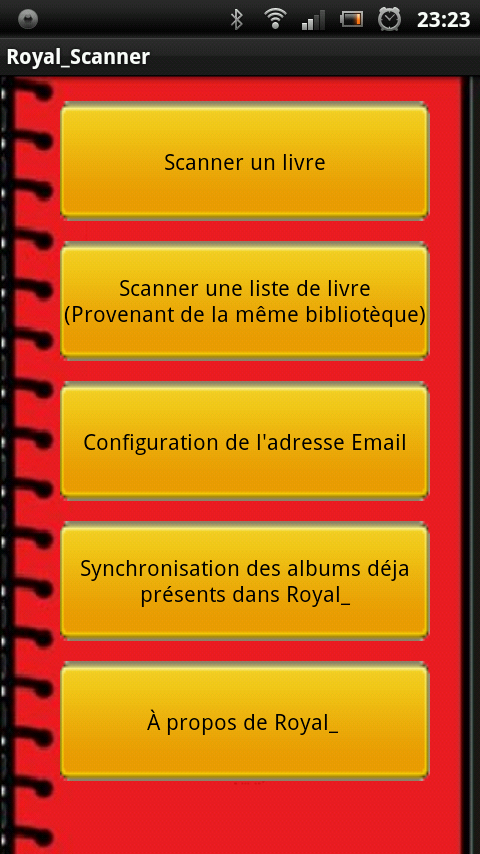
\includegraphics[height=7cm]{../Image_Royal_Scanner/Menu_Royal_Scanner.png}}
  \end{center}
\end{figure}

Sur c'est deux image nous pouvons voir la page de demarage de royal ainsi que le menu proposant les differentes fonctionnalitées de l'application Royal\_Scanner.


\begin{figure}[htbp]
  \begin{center}
    \leavevmode
    \subfloat[Capture en cours]{%
		\label{}
		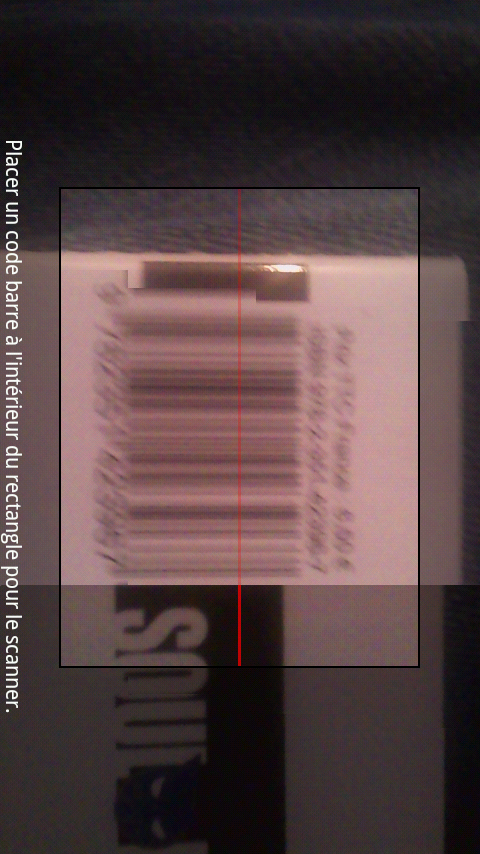
\includegraphics[height=7cm]{../Image_Royal_Scanner/Scan_En_Cours.png}}
    \hspace{4cm}
    \subfloat[Capture terminée]{%
		\label{}
		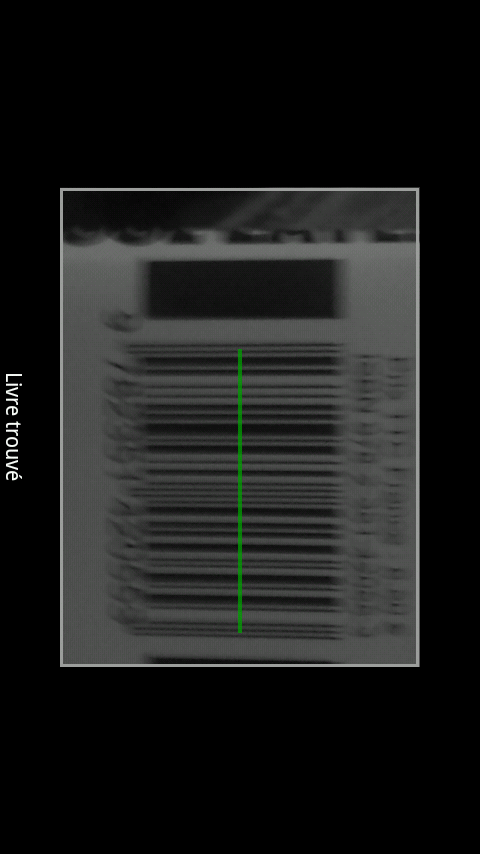
\includegraphics[height=7cm]{../Image_Royal_Scanner/Scan_Ok.png}}
  \end{center}
\end{figure}

Lorsqu'on lance une sequence de capture de code barre (simple ou multiple) un procedure basé sur la librarie Java ZXing qui permet la capture de code barre se lancera.
\newpage{}


\begin{figure}[htbp]
  \begin{center}
    \leavevmode
    \subfloat[Isbn correspondant valide (phase capture simple)]{%
		\label{}
		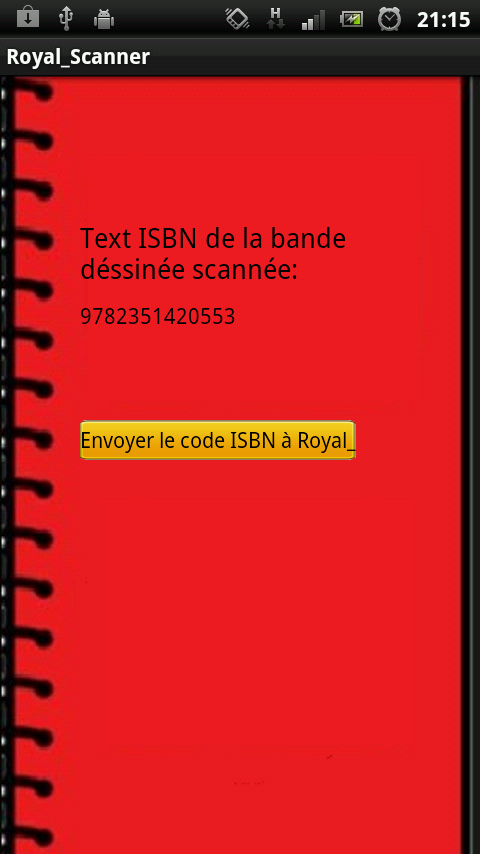
\includegraphics[height=7cm]{../Image_Royal_Scanner/Scan_Simple.png}}
    \hspace{1cm}
    \subfloat[Isbn correspondant non valide]{%
		\label{}
		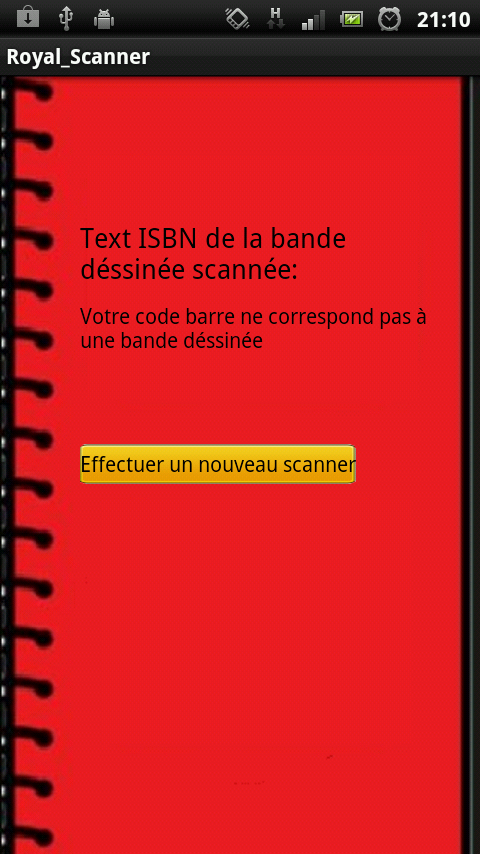
\includegraphics[height=7cm]{../Image_Royal_Scanner/Erreur_test_isbn.png}}
    \hspace{1cm}
    \subfloat[Isbn correspondant valide (phase capture multiple]{%
		\label{}
		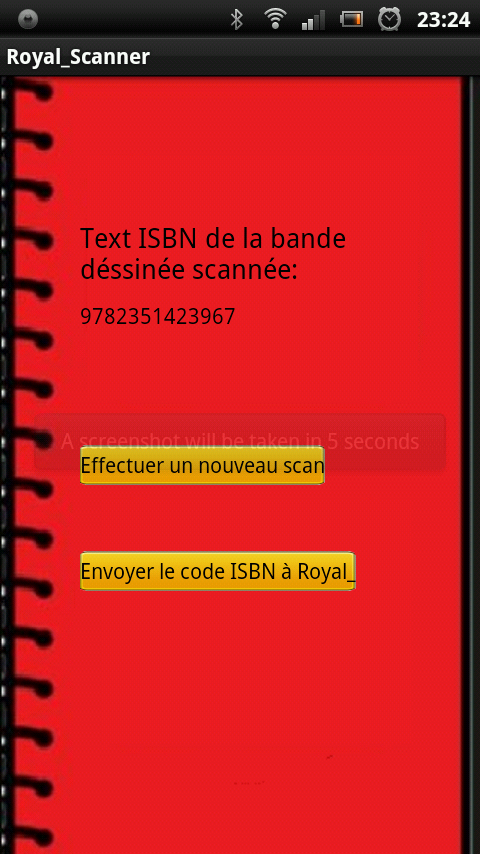
\includegraphics[height=7cm]{../Image_Royal_Scanner/Scan_Multiple.png}}
  \end{center}
\end{figure}

Après la procedure de capture l'application verifiera le code barre scanné.S'il est bon et que l'on est en capture simple l'application proposera la validation de l'album pour l'envoyer.
S'il est faut elle proposera un nouveau scan et enfin s'il est bon et que l(on est en capture multipple l'application proposera d'effectuer un nouveau scan ou d'envyer les ISBN des code barres capturés.

\begin{figure}[htbp]
  \begin{center}
    \leavevmode
    \subfloat[Configuration email page principal]{%
		\label{}
		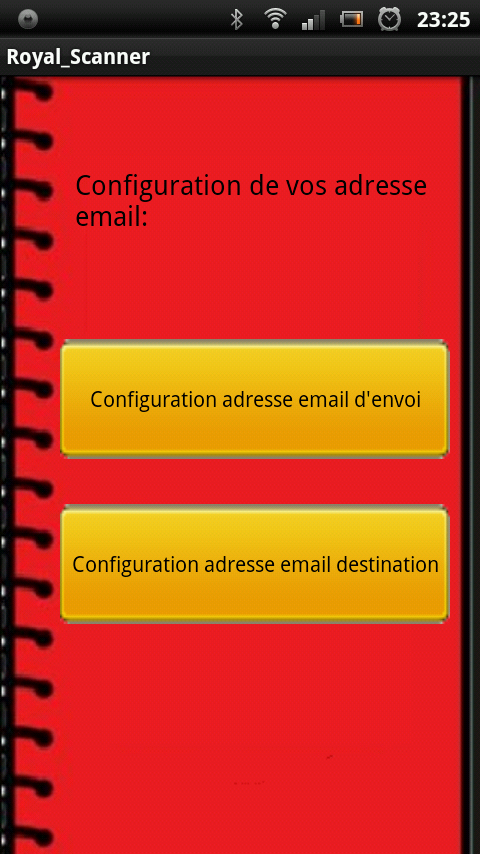
\includegraphics[height=7cm]{../Image_Royal_Scanner/Configue_Email_First_Page.png}}
    \hspace{4cm}
    \subfloat[Configuration email]{%
		\label{}
		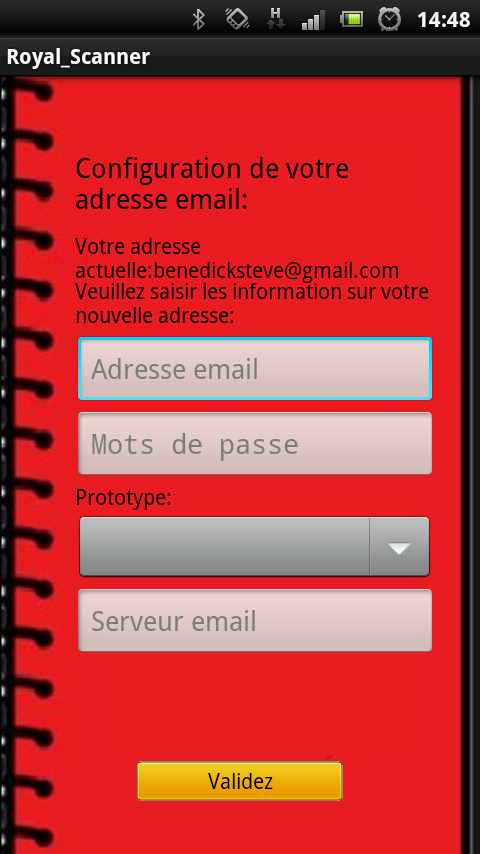
\includegraphics[height=7cm]{../Image_Royal_Scanner/Configue_Email.png}}
  \end{center}
\end{figure}

Lors de la configuration de l'adresse email nous pourrons configurer l'adresse utilisé afin d'envoyé l'email ainsi que l'adresse ou l'on envera les differents isbn.
\newpage{}

\begin{figure}[htbp]
  \begin{center}
    \leavevmode
    \subfloat[Synchronisation des albums déja present dans Royal\_]{%
		\label{}
		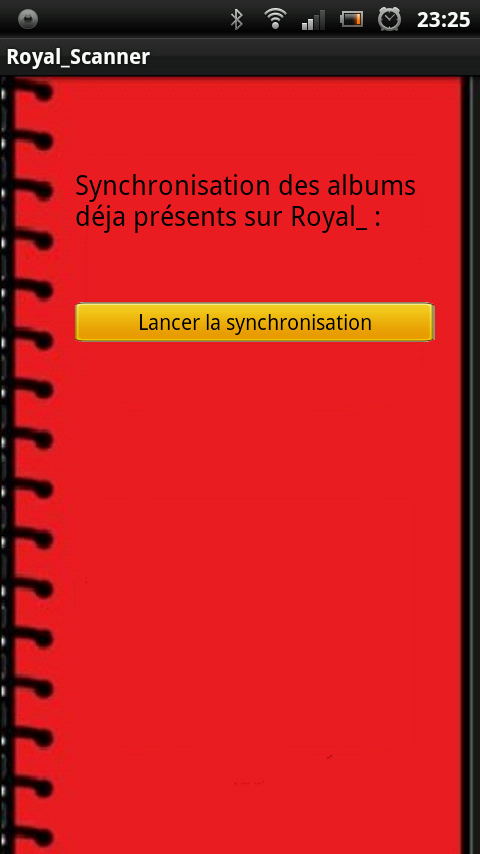
\includegraphics[height=7cm]{../Image_Royal_Scanner/Synchronisation_Album.png}}
    \hspace{4cm}
    \subfloat[Page à propos]{%
		\label{}
		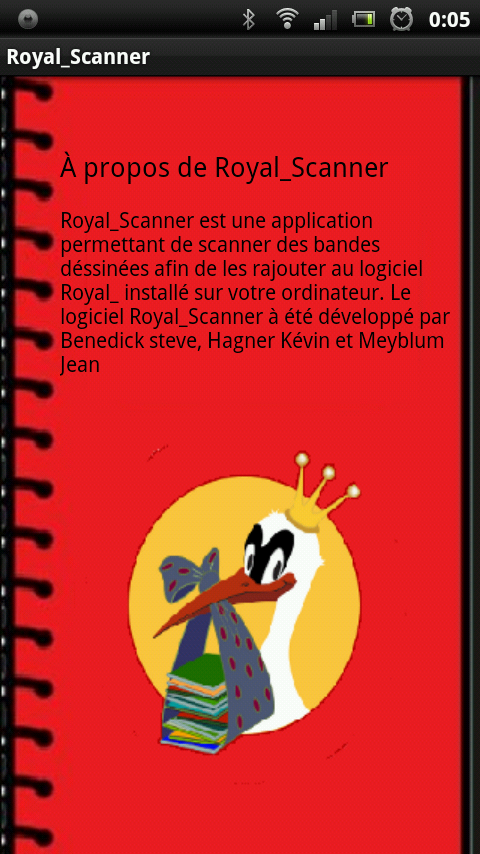
\includegraphics[height=7cm]{../Image_Royal_Scanner/A_Propos.png}}
  \end{center}
\end{figure}

Le prototype de la page de synchronisation n'est pas tres detailé car il s'agit d'une fonction de priorité 3 que l'on developpera plus tard dans le projet et que l'on definira la methode de transfere la plus performante une fois nos connaissance en developpement android plus grande. 
Cette page permettra sois la synchronisation par la recherche d'un email contenant tout les Isbn des album contenu dans royal soit la recuperation d'un fichier contenant c'est Isbn (fichier qui sera transmit soit par email soit directement par usb).
La page à propos permettera à l'utilisateur définira l'application.